
\subsection{Quantum Gates and Circuits}
\label{subsec:gates}

Quantum gates are the building blocks of quantum circuits. They are represented by \emph{unitary operators} \(U\) (i.e. \(U^\dagger U = I\)) that govern the evolution of quantum states. Key single-qubit gates include:
\begin{itemize}
    \item \textbf{Pauli-X (bit-flip):} 
    \[
    X = \begin{pmatrix} 0 & 1 \\ 1 & 0 \end{pmatrix},
    \]
    which acts as \(X|0\rangle = |1\rangle\) and \(X|1\rangle = |0\rangle\).
    \item \textbf{Hadamard (creating superpositions):}
    \[
    H = \frac{1}{\sqrt{2}}\begin{pmatrix} 1 & 1 \\ 1 & -1 \end{pmatrix}.
    \]
    \item \textbf{Phase shift:}
    \[
    R_\phi = \begin{pmatrix} 1 & 0 \\ 0 & e^{i\phi} \end{pmatrix}.
    \]
\end{itemize}

Two-qubit gates, such as the \textbf{Controlled-NOT (CNOT) gate}, introduce entanglement. The CNOT gate acts on a pair of qubits as
\[
\text{CNOT}|a\rangle|b\rangle = |a\rangle|a \oplus b\rangle,
\]
where \(\oplus\) denotes addition modulo 2.

Quantum circuits decompose complex algorithms into sequences of gate operations. A universal gate set (e.g., \(\{H, T, \text{CNOT}\}\)) can approximate any unitary operation to arbitrary precision, forming the basis for the quantum circuit model.

Figure~\ref{fig:deutsch_circuit} shows an example quantum circuit used in the Deutsch-Jozsa algorithm, illustrating the interplay of Hadamard gates and entangling operations.

\begin{figure}[h]
\centering
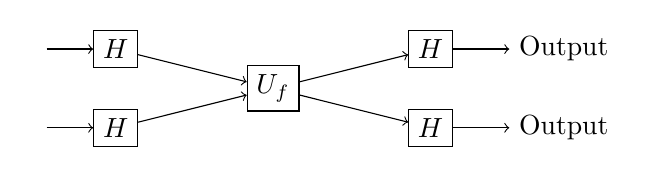
\begin{tikzpicture}[node distance=1.8cm, auto]
    \node (in1) at (0,0) {};
    \node (in2) at (0,-1) {};
    \node[draw, rectangle] (H1) at (1,0) {$H$};
    \node[draw, rectangle] (H2) at (1,-1) {$H$};
    \node[draw, rectangle] (Uf) at (3, -0.5) {\(U_f\)};
    \node[draw, rectangle] (H3) at (5,0) {$H$};
    \node[draw, rectangle] (H4) at (5,-1) {$H$};
    \draw[->] (in1) -- (H1);
    \draw[->] (in2) -- (H2);
    \draw[->] (H1) -- (Uf);
    \draw[->] (H2) -- (Uf);
    \draw[->] (Uf) -- (H3);
    \draw[->] (Uf) -- (H4);
    \draw[->] (H3) -- ++(1,0) node[right] {Output};
    \draw[->] (H4) -- ++(1,0) node[right] {Output};
\end{tikzpicture}
\caption{Quantum circuit for the Deutsch-Jozsa algorithm.}
\label{fig:deutsch_circuit}
\end{figure}
